% Four independent figures, each 88 x 70 mm, from the current FE500 dataset.
% build_convergence_fe500.py plots arithmetic means of matched runs 1--20.
% The legacy composite figure is not part of this manuscript input.
\begin{figure}[!tbp]
  \centering
  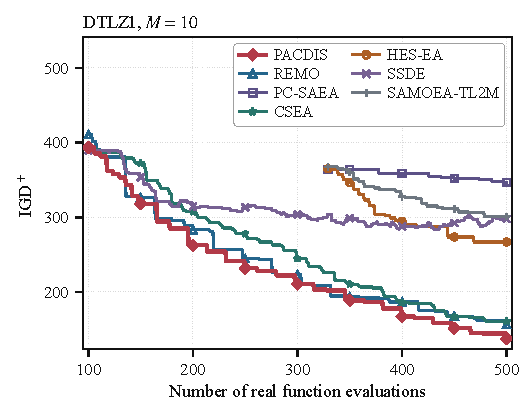
\includegraphics[width=88mm]{figures/fig_convergence_fe500_dtlz1_m10.pdf}
  \caption{Mean IGD$^+$ convergence on DTLZ1 ($M=10$, 20 runs). Curves
  hold saved values between checkpoints; the FE500 budget includes initialization.}
  \label{fig:exp:convergence:dtlz1}
\end{figure}

\begin{figure}[!tbp]
  \centering
  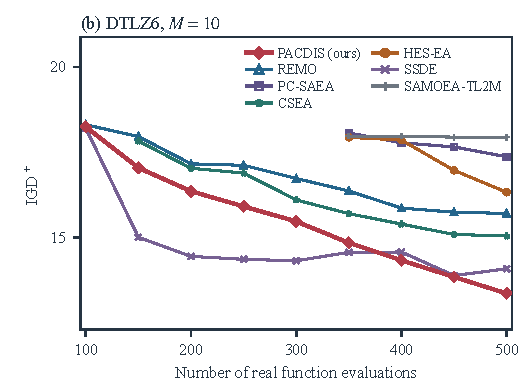
\includegraphics[width=88mm]{figures/fig_convergence_fe500_dtlz6_m10.pdf}
  \caption{Mean IGD$^+$ convergence on DTLZ6 ($M=10$, 20 runs). Curves
  hold saved values between checkpoints; the FE500 budget includes initialization.}
  \label{fig:exp:convergence:dtlz6}
\end{figure}

\begin{figure}[!tbp]
  \centering
  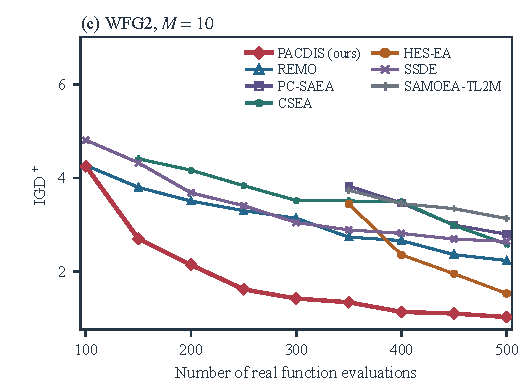
\includegraphics[width=88mm]{figures/fig_convergence_fe500_wfg2_m10.pdf}
  \caption{Mean IGD$^+$ convergence on WFG2 ($M=10$, 20 runs). Curves
  hold saved values between checkpoints; the FE500 budget includes initialization.}
  \label{fig:exp:convergence:wfg2}
\end{figure}

\begin{figure}[!tbp]
  \centering
  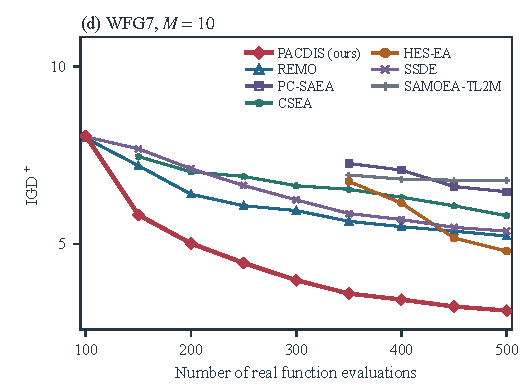
\includegraphics[width=88mm]{figures/fig_convergence_fe500_wfg7_m10.pdf}
  \caption{Mean IGD$^+$ convergence on WFG7 ($M=10$, 20 runs). Curves
  hold saved values between checkpoints; the FE500 budget includes initialization.}
  \label{fig:exp:convergence:wfg7}
\end{figure}
